%------------------------------------------------------------
%------------------------------------------------------------
\section{Introduction}
\label{sec:introduction}
%\todo[inline]{DL : Références générales : état de l'art timetabling}
L'organisation d'emplois du temps universitaires met en jeu des décisions d'ordre stratégique, tactique et opérationnel qui portent sur le maquettage des formations, la constitution des classes et groupes d'étudiants, l'affectation des services d'enseignement, le provisionnement de salles et d'équipements, et, in fine, la programmation des séances et des resources \cite{overview_uctp_2016_malaysian}.
Le périmètre de ces problèmes et le processus coordonnant leur résolution varie selon les pays et les institutions ainsi que le niveau d'automatisation et les sytèmes d'aide à la décision mis en oeuvre.
Au sein des universités françaises, par exemple, 
les maquettes de formation sont par convention revues tous les 5 ans et les étudiants s'inscrivent aux formations et personnalisent leurs parcours avant chaque période d'enseignement. 
Classes et groupes sont alors constitués selon les profils d'étudiants et les seuils d'effectifs par classe. 
Enseignants et salles sont ensuite positionnés sur les cours à dispenser avant que les séances de classe ne soient programmées et leurs ressources allouées (voir Figure~\ref{fig:utp-workflow}). 
Ce processus reste flexible (changements de personnels, etc.) et doit s'adapter aux impondérables qui rythment l'année universitaire (inscriptions tardives, absences, etc).

\begin{figure}[!t]
\begin{center}
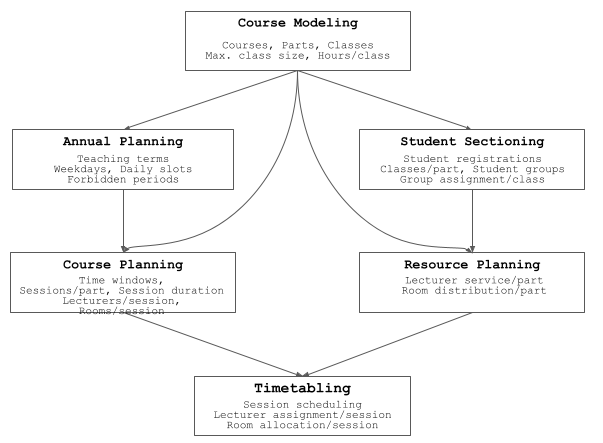
\includegraphics[width=\columnwidth]{2022_PATAT/img/utp_workflow.png}
\end{center}
\caption{Processus d'organisation d'emplois du temps}% dans le système universitaire français}
\label{fig:utp-workflow}
\end{figure}

Nous proposons dans cet article un langage de modélisation pour une classe étendue de problèmes d'emplois du temps universitaires ({\UTP}) se réduisant au problème de satisfaction de contraintes ({\CSP}).
Ce langage dédié permet de représenter différents aspects du problème relatifs au sectionnement de cours, la programmation de séances, la distribution de ressources et leur allocation
afin d'adapter chaque instance aux exigences de son environnement.
Le langage intègre un modèle formel et un langage de règles pour représenter entités et contraintes.
Le modèle d'entités s'appuie sur un horizon de temps multi-échelles (i.e. semaines, jours et créneaux quotidiens), 
un ensemble de ressources (i.e. étudiants, salles et enseignants),
et une structure hiérarchique de cours (i.e. cours, parties de cours, classes et séances).
Chaque séance est à programmer individuellement sur l'horizon de temps et les ressources nécessaires doivent lui être allouées.

Le modèle d'ordonnancement permet de représenter à la fois des séances mono-ressource et multi-ressources ainsi que des ressources disjonctives, cumulatives et hybrides.
D'une part, les séances sont étiquetées à ressource unique (p. ex. cours magistral) ou à ressources multiples (p. ex. cours hybride en distanciel et présentiel) en quantifiant le nombre de salles et d'enseignants requis.
Les étudiants se distribuent sur les cours selon leurs inscriptions alors que salles et enseignants se distribuent sur les parties de cours (p. ex. salles de travaux pratiques) ce qui détermine %indirectement 
le domaine des ressources allouables à chaque séance.
La charge de service est configurable pour les enseignants (i.e. nombre de séances à dispenser par partie de cours) et le volume de séances est figé pour les étudiants selon leur profil (i.e. toute partie de cours est obligatoire) tandis que les salles peuvent être utilisées à volonté.

L'utilisation simultanée d'une ressource n'est contrainte que pour les salles qui ont une capacité d'accueil indépassable, sauf dans le cas particulier des séances multi-salles qui s'appuient sur la capacité cumulée des salles allouées (p. ex. examen sur plusieurs salles).
Pour ce qui concerne la programmation des séances, chaque partie de cours possède sa propre grille horaire et chaque classe impose de séquencer ses séances dans un ordre prédéfini.
Chaque ressource peut donc être allouée à des séances se chevauchant (p. ex. classe obligatoire et tutorat) à l'exception des salles utilisées conjointement par une séance. 
Des règles peuvent être surimposées pour rendre des ressources, ou des classes de ressources, disjonctives.  
Enfin, le modèle impose de partitionner les étudiants en groupes et de ventiler les groupes sur les différentes classes en respectant des seuils d'effectifs et toute contrainte de sous-groupes posée entre classes.

Le langage de règles s'appuie sur un catalogue de prédicats qui permet d'exprimer des contraintes supplémentaires associant séances et entités.
Chaque contrainte porte sur une ou plusieurs paires, appelées e-maps, et éventuellement des paramètres selon le prédicat utilisé.
Une e-map associe une entité à un sous-ensemble de séances compatibles
et s'interprète comme une affectation conditionnelle. 
Autrement dit, 
une contrainte ne s'évalue que sur les séances pour lesquelles e-map(s) et solution considérée concordent, c'est-à-dire proposent la même entité. 
Chaque prédicat peut s'appliquer indistinctement à des ressources ou des éléments de cours.
Les e-maps peuvent donc être façonnées pour contraindre les séances allouables à une ressource (p. ex. indisponibilité d'un enseignant), les séances constitutives d'un élément de cours (p. ex. périodicité d'une classe), ou des séances individuelles (p. ex. parallélisation).
À noter que les contraintes portant sur des éléments de cours sont
de facto inconditionnelles.
%\marc{Modifier la fig4 pour rajouter les contraintes en plus des règles. Ajouter un texte à la fin de ce paragraphe et du suivant.}
La Figure~\ref{fig:utp-rule-1} présente trois contraintes : \ref{constraint-example-1} et \ref{constraint-example-2} portant chacune sur 2 classes, et \ref{constraint-example-3} portant sur un enseignant.
La contrainte \ref{constraint-example-3} porte sur 4 séances mais ne s'appliquera pas qu'à celles qui seront finalement affectées à l'enseignant.

Plutôt que de poser des contraintes individuelles, les règles sont utilisées pour formuler des conjonctions de contraintes ciblant des classes d'entités et de séances (p. ex. règles disjonctives sur enseignants, restrictions temporelles sur un cursus).
Chaque règle est liée à un prédicat et se définit par une contrainte quantifiée dont les quantificateurs restreignent le domaine de chaque variable e-map du prédicat.
Un langage de sélecteurs est fourni pour construire et filtrer les domaines d'e-maps par rang de séances, identifiant et type d'entités, ou toute classe d'éléments étiquettés par l'utilisateur (p. ex., équipe enseignante, bloc de salles).
Une règle dénote donc la conjonction de contraintes résultant de l'instanciation du prédicat sur le produit cartésien des domaines de variables.
% Ajout de l'exemple :
La Figure~\ref{fig:utp-rule-1} décrit les contraintes générées à partir de 2 règles : 
les contraintes \ref{constraint-example-1} et \ref{constraint-example-2} résultent de la règle \ref{rule-example-1} et la contrainte \ref{constraint-example-3} de la règle \ref{rule-example-2}.

\begin{figure}[!t]
\begin{center}
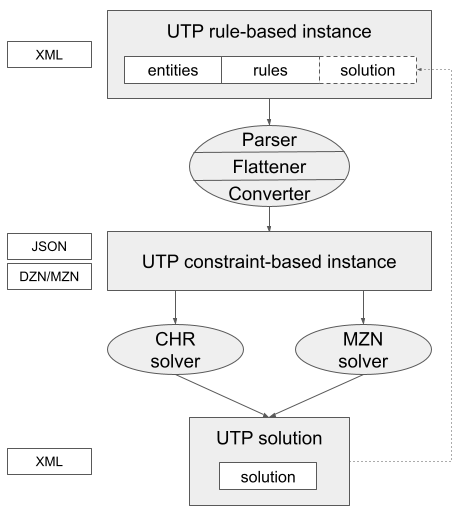
\includegraphics[scale=0.4]{2022_JFPC/img/utp_toolchain.png}
\end{center}
\caption{Chaîne de traitements {\UTP}}% dans le système universitaire français}
\label{fig:utp-toolchain}
\end{figure}

Le langage {\UTP} est implémenté sous la forme d'un langage {\XML}.
%et %et est embarqué \davidg{embarqué ? si c'est ce qui se dit dans le domaine, oubliez cette remarque} 
%dans les langages de modélisation par contraintes {\MINIZINC} \cite{MZN} et {\CHR} \cite{%Fruhwirth_TechReport_92}.
%Fruhwirth_CP_94}. %,Fruhwirth_JLP_98,Fruhwirth_CHR_09,Fruhwirth_Abdennadher_CHR_03,Fruhwirth_Raiser_2011}  
L'implémentation comprend un schéma {\XML} validant l'encodage d'instances %{\UTP} 
à base de règles et une chaîne de traitements comportant
un parseur {\XML},
un générateur transformant les règles en contraintes, 
et un encodeur convertissant les instances résultantes
dans un format approprié pour les solveurs (voir Figure~\ref{fig:utp-toolchain}).
L'intégration d'un solveur suppose d'implanter le modèle et les prédicats du langage {\UTP} et nous fournissons à cet effet deux implémentations alternatives en {\MINIZINC} \cite{MZN} et {\CHR} \cite{Fruhwirth_CP_94}.
%Au-delà de {\MINIZINC} et {\CHR}, les instances peuvent alimenter tout solveur implémentant le modèle, le format de solutions et les prédicats du langage.

%Nous présentons ici brièvement le langage {\UTP}, détaillons les modèles {\MINIZINC} et {\CHR} et présentons des expérimentations préliminaires menées sur un cas concret. %\davidg{je trouve que cette phrase fait redite avec l'annonce du plan qui est juste après}
%le premier cycle d'études dans une université française (licence). 
%Nous renvoyons le lecteur à \cite{uspSite} pour une spécification de l'encodage {\XML} qui fournit aussi l'accès aux codes sources des modèles {\MINIZINC} et {\CHR}, aux outils, et à un benchmark d'instances.
La suite de l'article s'organise comme suit.
Nous présentons brièvement le langage {\UTP} et dressons une comparaison à l'état de l'art en section~\ref{sec:langage-utp}.
%La section~\ref{sec:langage-utp} présente le langage {\UTP} et dresse une comparaison avec l'état de l'art.
%, notamment le schéma de représentation proposé dans le cadre de la compétition internationale {\ITC} \cite{ITC2019,2018muller}.
La section~\ref{sec:model} détaille les modèles de programmation par contraintes implémentés en {\MINIZINC} et {\CHR}.
La section~\ref{sec:experimentations} présente les premiers résultats expérimentaux.
La section~\ref{sec:conclusion} conclut et présente les perspectives envisagées pour la suite de ce travail.

